\section{Especificação da arquitetura do sistema}
\label{sec:requisitos_infra}

A arquitetura especificada neste trabalho define a organização técnica da solução proposta para comunicação, encaminhamento e persistência dos dados produzidos na rede de campo. Sua função é estruturar, de forma coerente, os componentes responsáveis pela coleta das informações, pela transição entre a comunicação embarcada e a infraestrutura de aplicação, e pelo armazenamento dos dados necessários ao funcionamento do sistema e às etapas posteriores de segurança e análise.

A solução foi organizada em quatro blocos principais: nó sensor, \textit{gateway}, \textit{backend} com API e persistência. No trecho de campo, o nó coleta os dados do ambiente e transmite quadros curtos por um enlace LoRa ponto a ponto, atendendo aos requisitos de operação em dispositivos com restrição energética. O \textit{gateway} concentra em um único dispositivo os papéis que o modelo LoRaWAN distribui entre \textit{gateway}, \textit{network server} e \textit{application server}: recebe os quadros, verifica a autenticidade e a ordem, registra os metadados de recepção e encaminha as mensagens ao \textit{backend}, em conformidade com os requisitos RF3, RF6 e RF12.

A partir do \textit{gateway}, a comunicação passa a utilizar Wi-Fi e requisições HTTP, integrando a rede embarcada a uma API autenticada e a um mecanismo centralizado de persistência, implantados em infraestrutura local, na mesma rede do \textit{gateway}. Essa escolha mantém a coleta independente de conectividade externa e dispensa a negociação de certificados no dispositivo embarcado; a migração para infraestrutura em nuvem, com transporte cifrado, é tratada como extensão e discutida no Capítulo~\ref{cap:consideracoes}. A camada de aplicação permanece disponível de forma contínua para o recebimento dos dados encaminhados pelo \textit{gateway}, e o próprio \textit{gateway} mantém os quadros em memória quando a API está indisponível.

Além dos dados de aplicação, como temperatura e luminosidade, a arquitetura prevê a persistência de metadados relevantes para o acompanhamento da comunicação, incluindo informações de origem, sequência, recepção e qualidade do enlace. Essa escolha atende aos requisitos RF5 e RF7 e contribui para a rastreabilidade da operação, conforme estabelecido em RNF6. Cada registro carrega ainda o identificador da sessão em que foi recebido e a indicação de ter sido entregue em tempo real ou reenviado após uma falha de conectividade (RF9 e RF10), de modo que uma queda da rede entre \textit{gateway} e \textit{backend} nunca se confunda com perda no enlace de rádio. A mesma base persistida prepara a infraestrutura para a incorporação de mecanismos de criptografia leve e de análise por aprendizado de máquina, em conformidade com RNF7 e RNF8.

A Figura~\ref{fig:arquitetura-especificada} apresenta a arquitetura técnica especificada para o sistema. A partir dessa organização, as subseções seguintes detalham os requisitos funcionais e não funcionais da infraestrutura proposta, que fundamentam e justificam as decisões arquiteturais adotadas.

\begin{figure}[htb]
  \caption{\label{fig:arquitetura-especificada}Arquitetura especificada do sistema proposto.}
  \begin{center}
      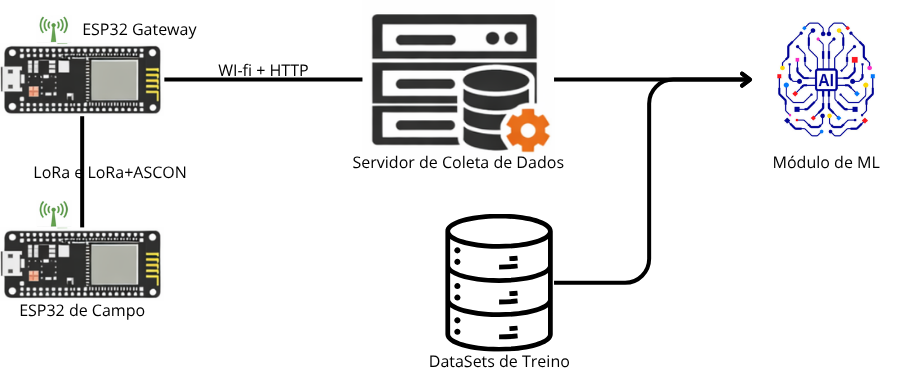
\includegraphics[scale=0.5]{barea/figuras/arch_figure1.png}
  \end{center}

\end{figure}

%%%%%%%%%%%%%%%%%%%%%%%%%%%%%%%%%%%%%%%%%%%%%%%%%%%%

\subsection{Requisitos funcionais da infraestrutura proposta}

Os requisitos funcionais da infraestrutura proposta descrevem os comportamentos esperados da arquitetura do sistema, considerando a coleta, o encaminhamento, a autenticação e a persistência das informações produzidas na rede de campo.

\begin{enumerate}
    \item[RF1.] O sistema deve permitir que os nós de campo coletem e transmitam dados de aplicação, incluindo, no protótipo previsto, informações de temperatura e luminosidade.

    \item[RF2.] Cada mensagem transmitida pelos nós deve conter, além dos dados de aplicação, informações mínimas de identificação e acompanhamento, incluindo identificador do dispositivo e contador de mensagens.

    \item[RF3.] O gateway deve receber as mensagens provenientes da rede de campo, registrar os metadados de recepção e encaminhar essas informações ao backend por meio de rede Wi-Fi e requisições HTTP.

    \item[RF4.] O backend deve autenticar as requisições enviadas pelo gateway, restringindo o recebimento de dados a dispositivos previamente autorizados.

    \item[RF5.] O sistema deve persistir os dados de aplicação recebidos dos nós juntamente com os metadados associados à comunicação.

    \item[RF6.] A infraestrutura deve permitir armazenamento temporário das mensagens no gateway em situações de indisponibilidade da conexão com o backend, com possibilidade de reenvio posterior.

    \item[RF7.] Os dados persistidos devem permanecer disponíveis para uso posterior pelas camadas de segurança e de análise por aprendizado de máquina.

    \item[RF8.] O gateway deve registrar cada quadro recebido em sua interface serial, em formato legível por máquina, independentemente do estado da conexão com o backend, de modo que a coleta nunca dependa da rede.

    \item[RF9.] O sistema deve identificar sessões de operação, de modo que quadros recebidos após um reinício do nó ou do gateway não sejam confundidos com a continuação da sequência anterior.

    \item[RF10.] Cada quadro persistido deve indicar sua origem: entregue em tempo real, reenviado a partir do armazenamento temporário do gateway ou relido de um registro serial.

    \item[RF11.] O gateway deve emitir periodicamente um sinal de vida com contadores de quadros recebidos, rejeitados e encaminhados, para distinguir ausência de tráfego de falha do próprio gateway.

    \item[RF12.] O gateway deve descartar, sem encaminhar, quadros com tamanho diferente do esperado, com falha de verificação de integridade, com falha de autenticação ou com contador não crescente, contabilizando cada caso separadamente.

\end{enumerate}

%%%%%%%%%%%%%%%%%%%%%%%%%%%%%%%%%%%%%%%%%%%%%%%%%%%%

\subsection{Requisitos não funcionais da infraestrutura proposta}

Os requisitos não funcionais da infraestrutura proposta descrevem propriedades de operação e restrições que devem ser observadas para que a solução seja compatível com o contexto de sistemas embarcados e Internet das Coisas. Para sua elicitação e organização, adotou-se como referência a norma ISO/IEC 25010, considerando principalmente características relacionadas à eficiência de desempenho, confiabilidade, compatibilidade, manutenibilidade e segurança.

\begin{enumerate}
    \item[RNF1.] A infraestrutura deve ser compatível com a operação de nós de campo com restrições de energia, priorizando baixo consumo no trecho embarcado da comunicação.

    \item[RNF2.] A comunicação do sistema deve ser orientada a evento, evitando transmissões contínuas desnecessárias entre os componentes.

    \item[RNF3.] A arquitetura deve manter separação clara entre a rede de campo, baseada em LoRa ponto a ponto, e a infraestrutura de aplicação, baseada em Wi-Fi e HTTP, de modo que a recepção de rádio nunca aguarde a rede.

    \item[RNF4.] O protótipo deve preservar simplicidade de integração entre hardware, comunicação e backend, de modo a manter viável sua montagem e evolução no contexto do projeto.

    \item[RNF5.] A infraestrutura deve apresentar robustez básica a falhas temporárias de conectividade entre gateway e backend.

    \item[RNF6.] O sistema deve garantir rastreabilidade das mensagens recebidas, por meio do registro de dados e metadados que permitam identificar origem, sequência, instante de recepção e condições básicas do enlace.

    \item[RNF7.] A arquitetura deve ser compatível com a incorporação posterior de mecanismos de criptografia leve sem exigir reformulação completa da infraestrutura de comunicação.

    \item[RNF8.] A infraestrutura deve ser compatível com o uso posterior de técnicas de aprendizado de máquina aplicadas à análise do comportamento da rede e à detecção de anomalias.
    
    \item[RNF9.] O quadro transmitido não deve exceder 51 bytes, limite do plano regional AU915 na taxa de dados mais lenta, de modo que possa ser transmitido em qualquer fator de espalhamento.

    \item[RNF10.] Os metadados de recepção registrados devem ter os mesmos campos e a mesma semântica das variáveis candidatas dos modelos de detecção, permitindo comparar a coleta própria com o conjunto de dados de referência sem transformação adicional.

    \item[RNF11.] O envio ao backend não deve bloquear a recepção de rádio: um quadro que chegue durante uma requisição HTTP em andamento deve ser recebido e registrado normalmente.

\end{enumerate}

%%%%%%%%%%%%%%%%%%%%%%%%%%%%%%%%%%%%%%%%%%%%%%%%%%%%

\subsection{Rastreabilidade dos requisitos da infraestrutura}
\label{subsec:rastreabilidade_infra}

A Tabela~\ref{tab:rastreabilidade_infra} relaciona cada requisito ao componente que o atende e à forma como foi verificado. Os detalhes de implementação estão no Capítulo~\ref{cap:desenvolvimento}. As evidências vêm das quatro coletas em bancada (23 de agosto, 24 de setembro, 8 de outubro e 12 a 13 de outubro de 2026), das cinco suítes de teste executadas nas placas e dos testes automatizados do \textit{backend}. Dois requisitos estão atendidos apenas em parte e são declarados como tal: o RF1, porque os dados de aplicação ainda são sintéticos; e o RNF1, porque o nó ainda não entra em modo de baixo consumo entre transmissões. O RF6, declarado parcial até outubro, foi exercitado em uma queda real de rede em 13 de outubro.

\begin{table}[!htbp]
\centering
\caption{Rastreabilidade dos requisitos da infraestrutura}
\label{tab:rastreabilidade_infra}
\footnotesize
\begin{tabular}{lp{5,2cm}p{8cm}}
\hline
\textbf{Req.} & \textbf{Onde é atendido} & \textbf{Como foi verificado} \\
\hline
RF1  & Firmware do nó; 4 bytes de dados no quadro & Quatro coletas, de 23/08 a 13/10; dados sintéticos (parcial) \\
RF2  & Cabeçalho do quadro: identificador e contador & Suítes do quadro v2 (14 casos) e v3 (14 casos) na placa; coletas \\
RF3  & Gateway: recepção no núcleo 1, envio HTTP no núcleo 0 & 6.007 quadros recebidos em 12 a 13/10, 2.432 entregues ao vivo \\
RF4  & Token no cabeçalho HTTP, comparação em tempo constante & Testes automatizados do backend \\
RF5  & Banco SQLite com os 12 campos e metadados de ingestão & Testes; conferência serial contra banco \\
RF6  & Fila e armazenamento temporário de 512 registros no gateway & Queda real do Wi-Fi em 13/10: 512 retidos, os mais antigos descartados como previsto \\
RF7  & API de consulta e exportação em CSV & Ferramenta de análise; notebooks \\
RF8  & Registro serial sob exclusão mútua, anterior ao envio & Coleta de 23/08 sem backend; 3.575 quadros recuperados do registro em 13/10 \\
RF9  & Identificador de sessão: sorteio na inicialização mais contador de sessão & Suíte do gateway na placa; uma sessão distinta por coleta \\
RF10 & Campo de origem por idade do registro na entrega & 13/10: 2.432 ao vivo e 3.575 relidos do registro serial, distinguidos no banco \\
RF11 & Sinal de vida a cada 30 s na serial e na API & Registro serial; 669 sinais de vida no banco desde 08/10 \\
RF12 & Verificação de tamanho, CRC, anti-replay e tag & Suítes v2 e v3 na placa: forjado, repetido e contador alto rejeitados; 0 rejeições indevidas em 6.468 quadros \\
RNF1 & Potência de 5 dBm; nó sem modo de repouso & Parcial: repouso entre transmissões pendente \\
RNF2 & Recepção por interrupção; transmissão periódica & Coletas \\
RNF3 & Dois núcleos com fila de espera zero & 0 perdas em 6.007 quadros com a tarefa de rede ativa \\
RNF4 & Contrato único compartilhado pelos dois firmwares & Compilação; testes \\
RNF5 & Armazenamento temporário e espera exponencial de 1 a 30 s & Queda de 13/10: gateway seguiu recebendo e tentando reenviar por 5 h \\
RNF6 & 12 campos mais identificadores de gateway, sessão e instante UTC & Conferência serial contra banco \\
RNF7 & Dois caminhos de cifra, selecionados em tempo de compilação & AES-GCM no ar em 24/09; Ascon-128a no ar desde 08/10 \\
RNF8 & Mesmos campos das variáveis candidatas dos modelos & Análise das coletas \\
RNF9 & Quadro de 26 bytes; verificação em tempo de compilação & Compilação \\
RNF10 & Formatação byte a byte do registro & Suíte do gateway na placa (16 casos, 17/11); ETL compara coleta própria e Tour Perret sem conversão \\
RNF11 & Fila entre núcleos com espera zero & 0 perdas em 6.007 quadros com envio HTTP concorrente \\
\hline
\end{tabular}
\legend{Fonte: elaborado pelos autores (2026).}
\end{table}


%%%%%%%%%%%%%%%%%%%%%%%%%%%%%%%%%%%%%%%%%%%%%%%%%%%%
%%%%%%%%%%%%%%%%%%%%%%%%%%%%%%%%%%%%%%%%%%%%%%%%%%%%
